% TAREA 1 PROGRA 2


\section*{Sipser}



% PROBLEMA 1.1
\begin{mdframed}[style = warning]
	\begin{problem}
		($1.1$) Respondiendo las preguntas para los autómatas dados:
			\begin{enumerate}[a)]
				\item El estado inicial de $M_1$ es $q_o = q_1$, y de $M_2$ es $q_o = q_1$.
				\item Los estados aceptados de $M_1$ es $F = \{ q_2 \}$ y de $M_2$ es $F = \{ q_1,q_4 \}$.
				\item La secuencia en $M_1$ es $q_1,q_2,q_3q_1,q_1$. Para $M_2$ es $q_1,q_1,q_1,q_2,q_4$.
				\item De dicha palabra, solo el automata $M_2$ lo acepta.
				\item La cadena vacía no es aceptada.
			\end{enumerate}
	\end{problem}
\end{mdframed}











% PROBLEMA 2.1
\begin{mdframed}[style = warning]
	\begin{problem}
		($1.3$) Para el automata dado, el diagrama de estado es:
		\begin{figure}[H]
			\centering
			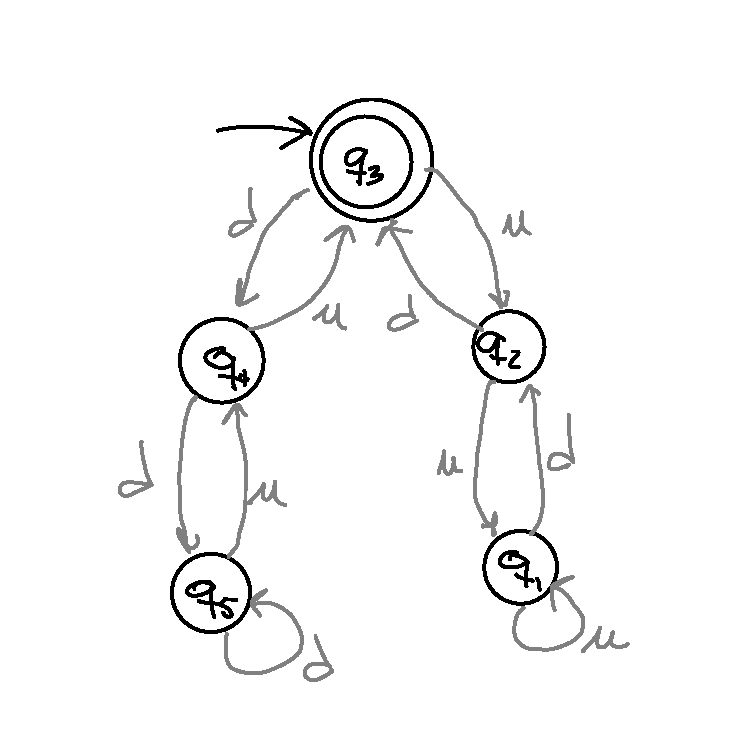
\includegraphics[scale=0.7]{Images/1-3.pdf}
			\caption{Diagrama de Estado, creado en \textit{Xournal}}
			\label{1-3}
		\end{figure}		 
	\end{problem}
\end{mdframed}












\begin{mdframed}[style = warning]
	\begin{problem}
		($1.4$) 	 
	\end{problem}
\end{mdframed}










\begin{mdframed}[style = warning]
	\begin{problem}
		($1.6$)
		\begin{enumerate}[a)]
			\item .
				\begin{figure}[H]
					\centering
					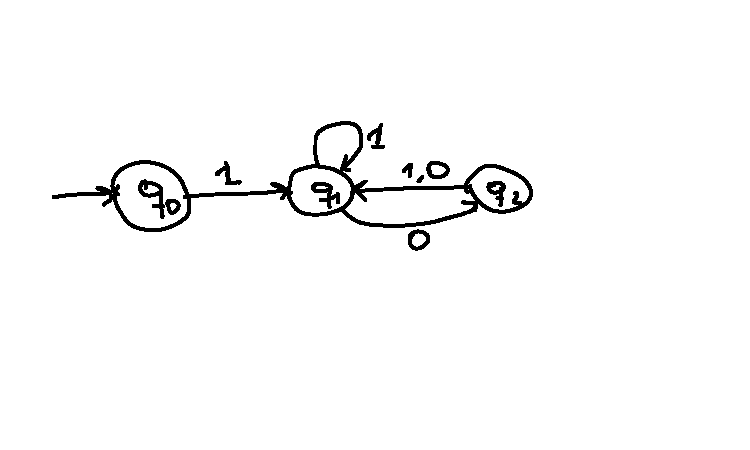
\includegraphics[scale=0.7]{Images/1-6-a.pdf}
					\caption{AFD, creado en \textit{Xournal}}
					\label{1-6-a}
				\end{figure}
				
			\item .
				\begin{figure}[H]
					\centering
					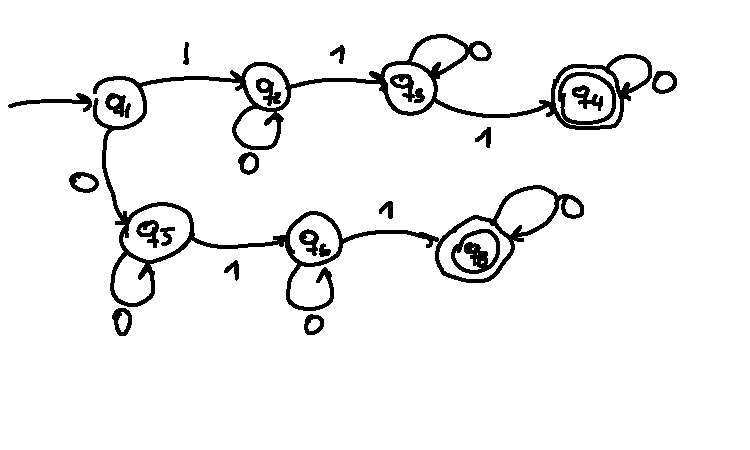
\includegraphics[scale=0.7]{Images/1-6-b.pdf}
					\caption{AFD, creado en \textit{Xournal}}
					\label{1-6-b}
				\end{figure}
				
			\item .
				\begin{figure}[H]
					\centering
					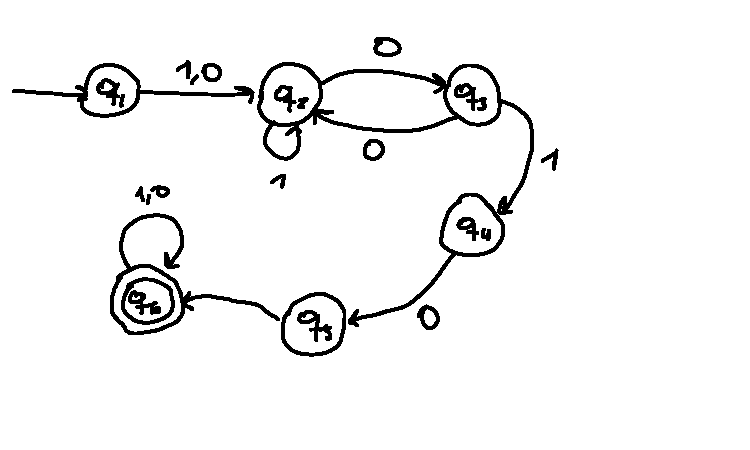
\includegraphics[scale=0.7]{Images/1-6-c.pdf}
					\caption{AFD, creado en \textit{Xournal}}
					\label{1-6-c}
				\end{figure}
				
			\item .		
				\begin{figure}[H]
					\centering
					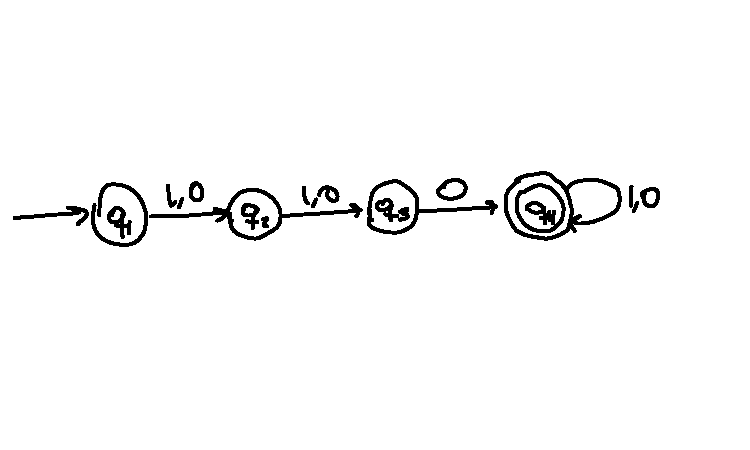
\includegraphics[scale=0.7]{Images/1-6-d.pdf}
					\caption{AFD, creado en \textit{Xournal}}
					\label{1-6-d}
				\end{figure}
				
			\item .		
				\begin{figure}[H]
					\centering
					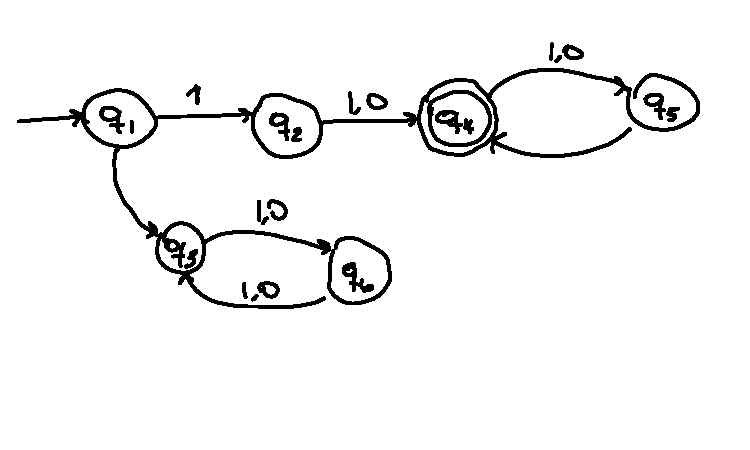
\includegraphics[scale=0.7]{Images/1-6-e.pdf}
					\caption{AFD, creado en \textit{Xournal}}
					\label{1-6-e}
				\end{figure}
				
			\item .		
				\begin{figure}[H]
					\centering
					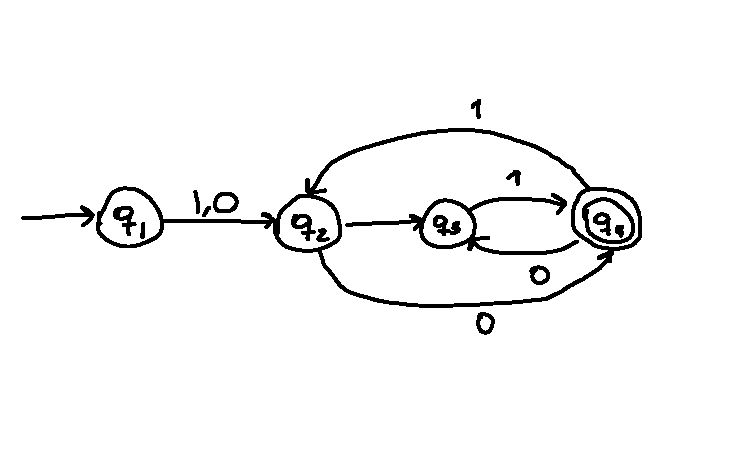
\includegraphics[scale=0.7]{Images/1-6-f.pdf}
					\caption{AFD, creado en \textit{Xournal}}
					\label{1-6-f}
				\end{figure}
				
			\item .		
				\begin{figure}[H]
					\centering
					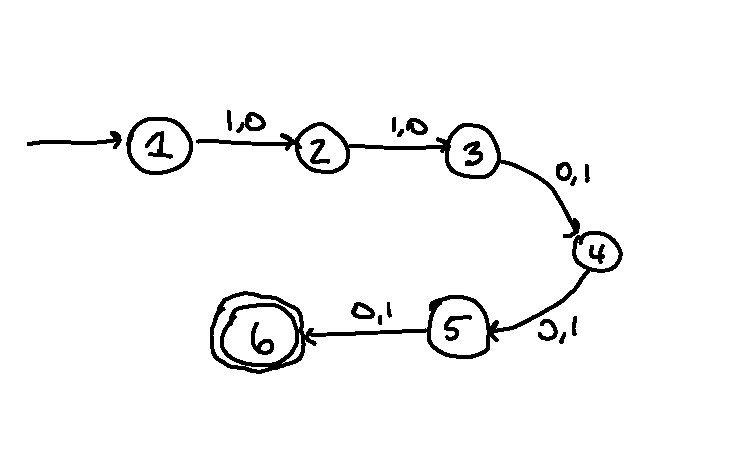
\includegraphics[scale=0.7]{Images/1-6-g.pdf}
					\caption{AFD, creado en \textit{Xournal}}
					\label{1-6-g}
				\end{figure}
				
			\item .		
				
				
			
			\item .		
				\begin{figure}[H]
					\centering
					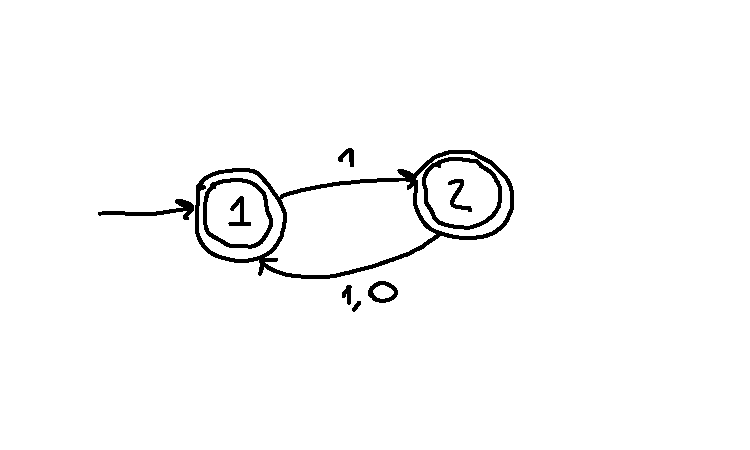
\includegraphics[scale=0.6]{Images/1-6-i.pdf}
					\caption{AFD, creado en \textit{Xournal}}
					\label{1-6-i}
				\end{figure}
				
			\item .		
				\begin{figure}[H]
					\centering
					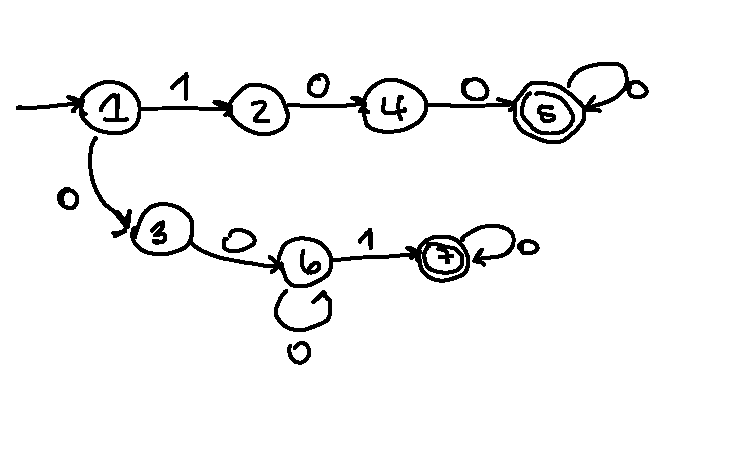
\includegraphics[scale=0.7]{Images/1-6-j.pdf}
					\caption{AFD, creado en \textit{Xournal}}
					\label{1-6-j}
				\end{figure}
				
				
			\item .		
				\begin{figure}[H]
					\centering
					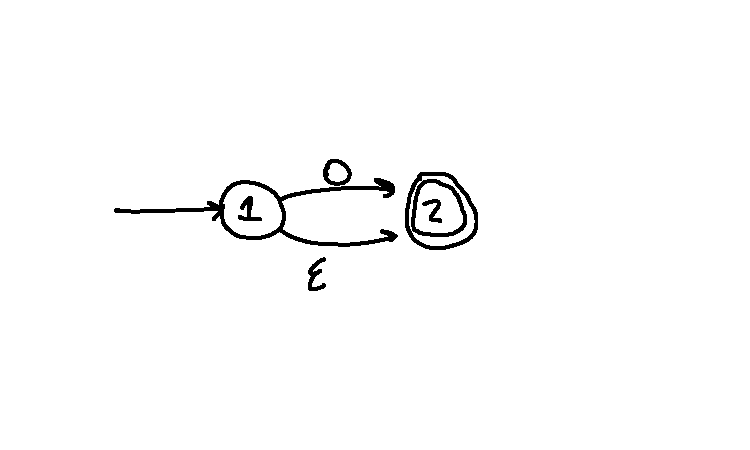
\includegraphics[scale=0.7]{Images/1-6-k.pdf}
					\caption{AFD, creado en \textit{Xournal}}
					\label{1-6-k}
				\end{figure}
				
			\item .	
			\item .		
				\begin{figure}[H]
					\centering
					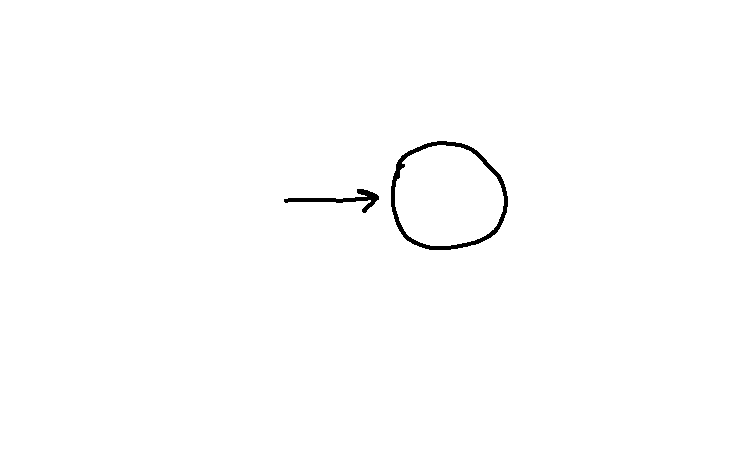
\includegraphics[scale=0.7]{Images/1-6-m.pdf}
					\caption{AFD, creado en \textit{Xournal}}
					\label{1-6-m}
				\end{figure}
				
			\item .		
				\begin{figure}[H]
					\centering
					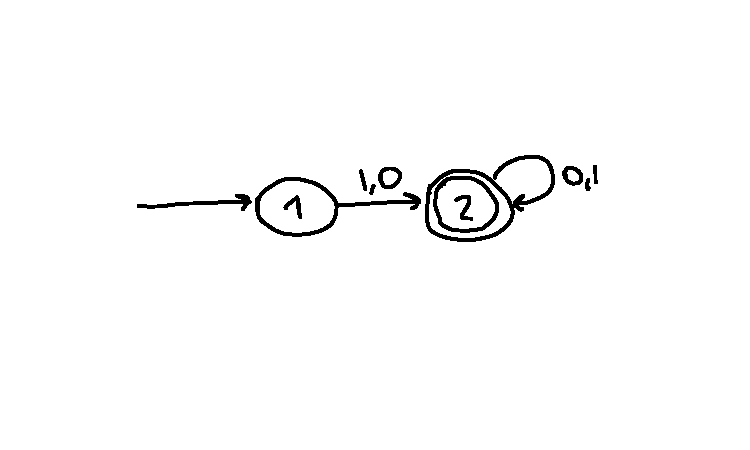
\includegraphics[scale=0.7]{Images/1-6-n.pdf}
					\caption{AFD, creado en \textit{Xournal}}
					\label{1-6-n}
				\end{figure}
		\end{enumerate}
	\end{problem}
\end{mdframed}









\begin{mdframed}[style = warning]
	\begin{problem}
		($1.8$)
		\begin{enumerate}[a)]
			\item Uniendo ambos lenguajes, simplemente tiene que iniciar con $1$ y terminar con $0$, además de tener como mínimo $3$ $1$'s.
			\begin{figure}[H]
				\centering
				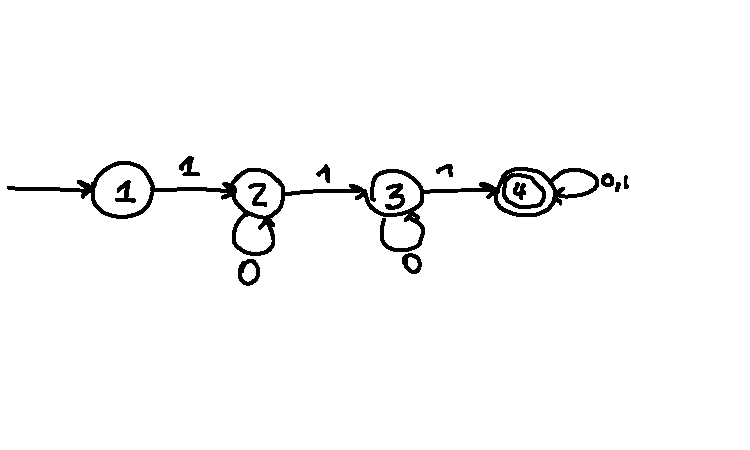
\includegraphics[scale=0.7]{Images/1-8-a.pdf}
				\caption{Union de Automatas, creado en \textit{Xournal}}
				\label{Union}
			\end{figure}
		\end{enumerate}		 
	\end{problem}
\end{mdframed}














\begin{mdframed}[style = warning]
	\begin{problem}
		($1.11$) Como la representación de los autómatas es de gráfos, la propiedad de contracción se debe cumplir, es decir que, al unir dos vértices en uno solo, se crea un nuevo grafo. Dichos dos vértices, pueden ser perfectamente, dos estados de aceptación, de modo que las aristas que los unen se eliminan, los bucles se unifican. Esto conservaría las mismas propiedades del autómata.
	\end{problem}
\end{mdframed}
















\begin{mdframed}[style = warning]
	\begin{problem}
		($1.12$) 	 
	\end{problem}
\end{mdframed}














\begin{mdframed}[style = warning]
	\begin{problem}
		($1.14$) 	 
	\end{problem}
\end{mdframed}











\begin{mdframed}[style = warning]
	\begin{problem}
		($1.16$) 
		\begin{enumerate}[a)]
			\item Para el automata dado, se tiene la siguiente función de transición referida a un automata determinista:
			\begin{table}[H]
				\centering
				\begin{tabular}{c|cc}
					 & $a$ & $b$ \\
					\hline
					$q_o \to \{ 1 \}$ & $\{ 1,2 \}$ & $\{ 2 \}$ \\
					$q_1 \to \{ 2 \}$ & $\emptyset$ & $\{ 1 \}$ \\
					$q_2 \to \{ 1,2 \}$ & $\{ 1,2 \}$ & $\{ 1,2 \}$
				\end{tabular}
			\end{table}
			La cual, en base al mismo alfabeto, y el conjunto de estados propuesto, se tienen los siguientes estados aceptados $F = \{ q_o ,q_2 \}$. De modo que el $AFD$ es
				\begin{figure}[H]
					\centering
					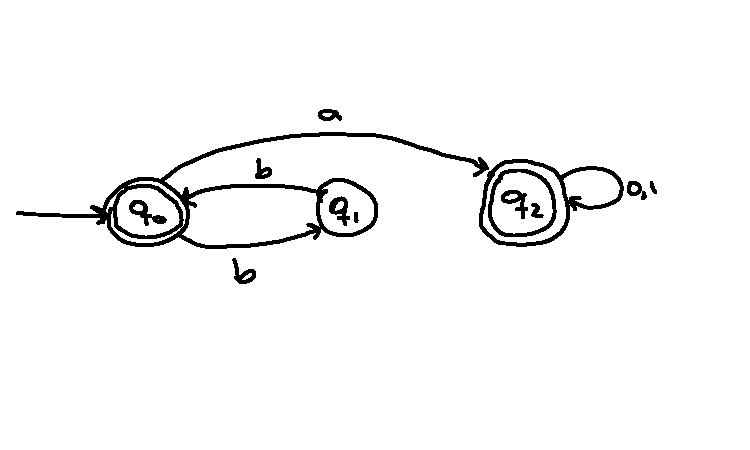
\includegraphics[scale=0.7]{Images/1-16-a.pdf}
					\caption{AFD asociado, creado con \textit{Xournal}}
					\label{16-a}
				\end{figure}
			\item Realizando lo mismo para este nuevo automata se tiene, que el estado inicial del AFD es $E(\{ 1 \}) = \{ 1,2 \}$, de modo que:
				\begin{table}[H]
					\centering
					\begin{tabular}{c|cc}
						 & $a$ & $b$ \\
						\hline
						$q_1 \to \{ 1 \}$ & $\{ 3 \}$ & $\emptyset$ \\
						$q_2 \to \{ 3 \}$ & $\{ 2 \}$ & $\{ 2,3 \}$ \\
						$q_3 \to \{ 2 \}$ & $\{ 1 \}$ & $\emptyset$ \\
						$q_4 \to \{ 2,3 \}$ & $\{ 1,2 \}$ & $\{ 2,3 \}$ \\
						$q_o \to \{ 1,2 \}$ & $\{ 3,1 \}$ & $\emptyset$ \\
						$q_5 \to \{ 1,3 \}$ & $\{ 2,3 \}$ & $\{ 2,3 \}$ 
					\end{tabular}
				\end{table}
			Lo que genera el siguiente AFD, con los estados de aceptacion $F = \{ q_o,q_3,q_3 \}$.
				\begin{figure}[H]
					\centering
					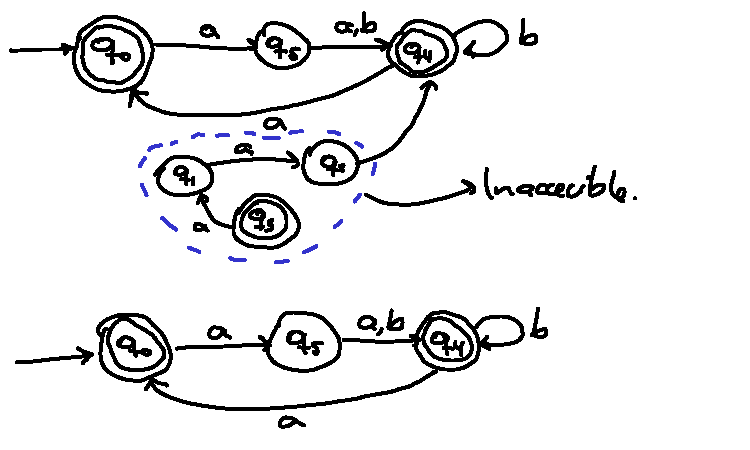
\includegraphics[scale=0.7]{Images/1-16-b.pdf}
					\caption{AFD asociado, creado con \textit{Xournal}}
					\label{16-b}
				\end{figure}
		\end{enumerate}
	\end{problem}
\end{mdframed}












\begin{mdframed}[style = warning]
	\begin{problem}
		($1.17$) 	
		\begin{enumerate}[a)]
			\item Dado $(01|001|010)^*$, se construye el AFND:
				\begin{figure}[H]
					\centering
					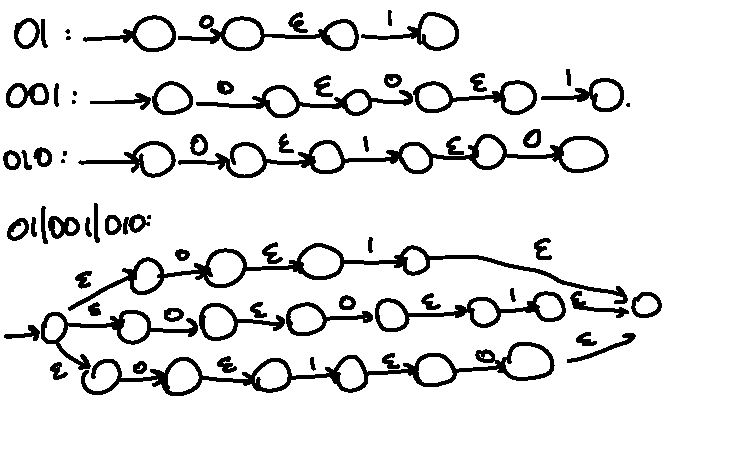
\includegraphics[scale=0.9]{Images/1-17-1a.pdf}
					\caption{Construcción del AFND, creado con \textit{Xournal}}
					\label{17-1a}
				\end{figure}
			De esto, se genera el AFND:
				\begin{figure}[H]
					\centering
					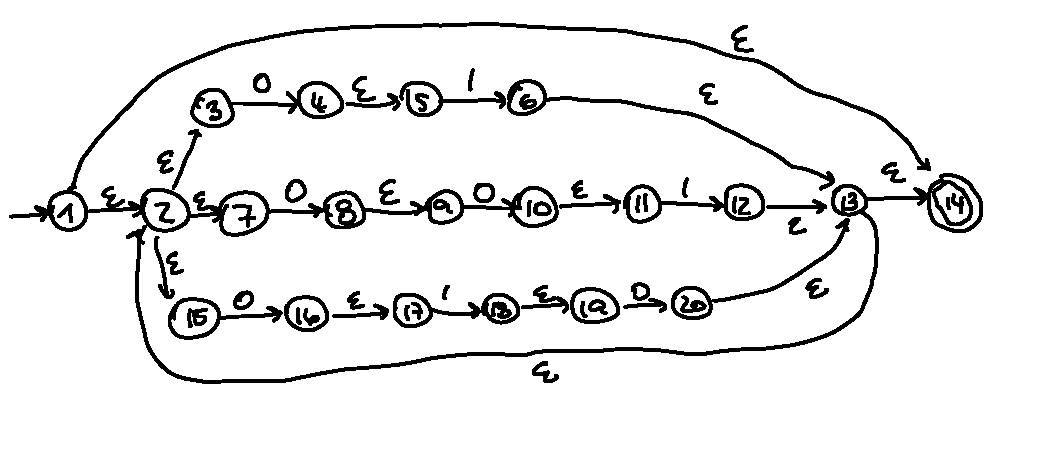
\includegraphics[scale=0.9]{Images/1-17-2a.pdf}
					\caption{AFND generado, creado con \textit{Xournal}}
					\label{17-2a}
				\end{figure}
			\item Tomando todas las $\varepsilon$ transiciones, unicamente se utiliza la que contenga al estado inicial del AFND, esto porque solo estas serán alcanzadas en el AFD. De modo que la nueva función de transición es:
				\begin{table}[H]
					\centering
					\begin{tabular}{c|cc}
						 & $a$ & $b$ \\
						\hline
						$q_o \to \{ 1,2,3,7,15,14 \}$ & $\{ 4,5,8,9,16,17 \}$ & $\emptyset$ \\
						$q_1 \to \{ 4,5,8,9,16,17 \}$ & $\{ 10,11 \}$ & $\{ 6,13,14,2,18,19 \}$ \\
						$q_3 \to \{ 10,11 \}$ & $\emptyset$ & $\{ 12,13,14,2 \}$ \\
						$q_5 \to \{ 6,13,14,2,18,19 \}$ & $\{ 20,13,14,2 \}$ & $\emptyset$ \\
						$q_5 \to \{ 12,13,14,2 \}$ & $\emptyset$ & $\emptyset$ \\
						$q_6 \to \{ 20,13,14,2 \}$ & $\emptyset$ & $\emptyset$ 
					\end{tabular}
				\end{table}
			El diagrama del AFD sería
				\begin{figure}[H]
					\centering
					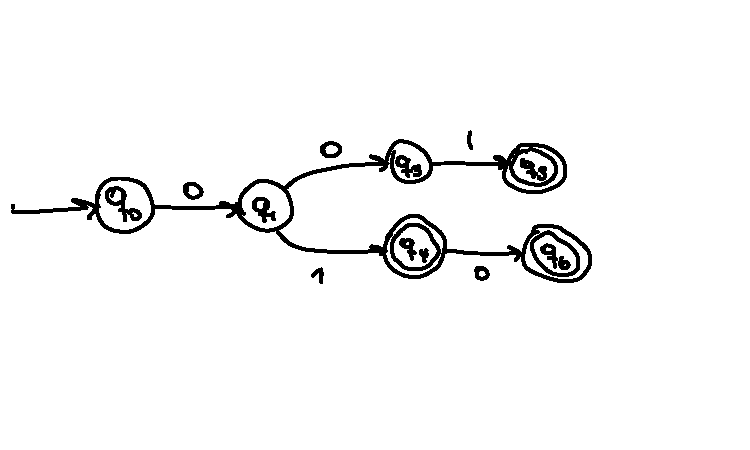
\includegraphics[scale=0.9]{Images/1-17-b.pdf}
					\caption{AFD generado, creado con \textit{Xournal}}
					\label{17-b}
				\end{figure}
		\end{enumerate}		 
	\end{problem}
\end{mdframed}










\begin{mdframed}[style = warning]
	\begin{problem}
		($1.19$) 	 
		\begin{enumerate}[a)]
			\item Para $(0|1)^*000(0|1)^*$, se crea el AFND.
				\begin{figure}[H]
					\centering
					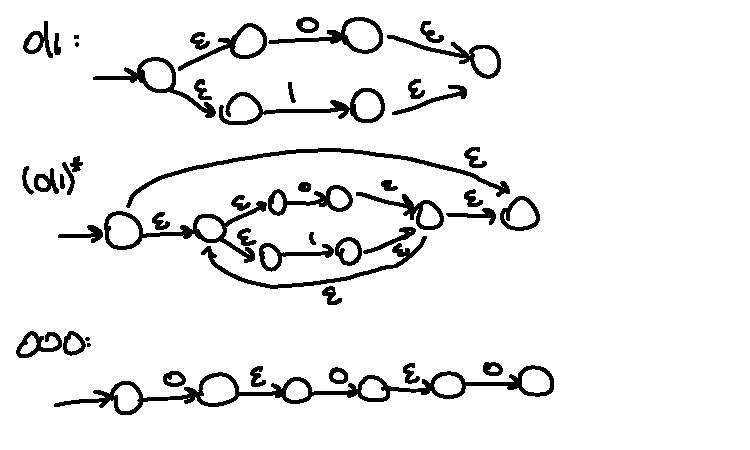
\includegraphics[scale=0.9]{Images/1-19-1a.pdf}
					\caption{Construcción del AFND, creado con \textit{Xournal}}
					\label{19-1a}
				\end{figure}
			Lo que lleva a:
				\begin{figure}[H]
					\centering
					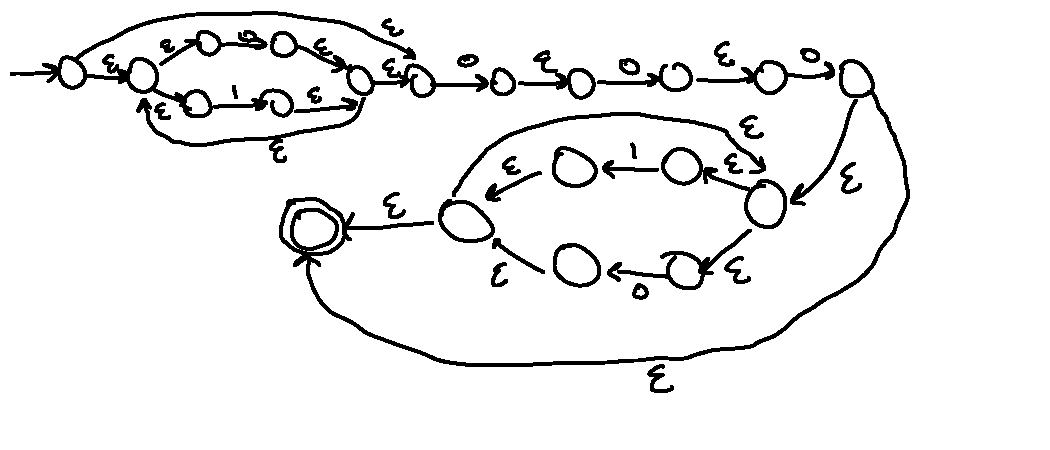
\includegraphics[scale=0.9]{Images/1-19-2a.pdf}
					\caption{AFND, creado con \textit{Xournal}}
					\label{19-2a}
				\end{figure}
			\item Para $(((00)^*(11))|01)^*$, se crea el AFND.
				\begin{figure}[H]
					\centering
					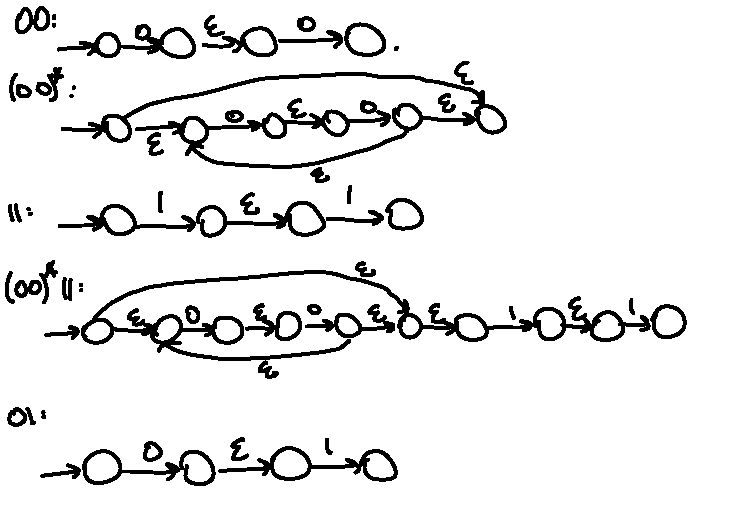
\includegraphics[scale=0.9]{Images/1-19-1b.pdf}
					\caption{Construcción del AFND, creado con \textit{Xournal}}
					\label{19-1b}
				\end{figure}
			Lo que lleva a:
				\begin{figure}[H]
					\centering
					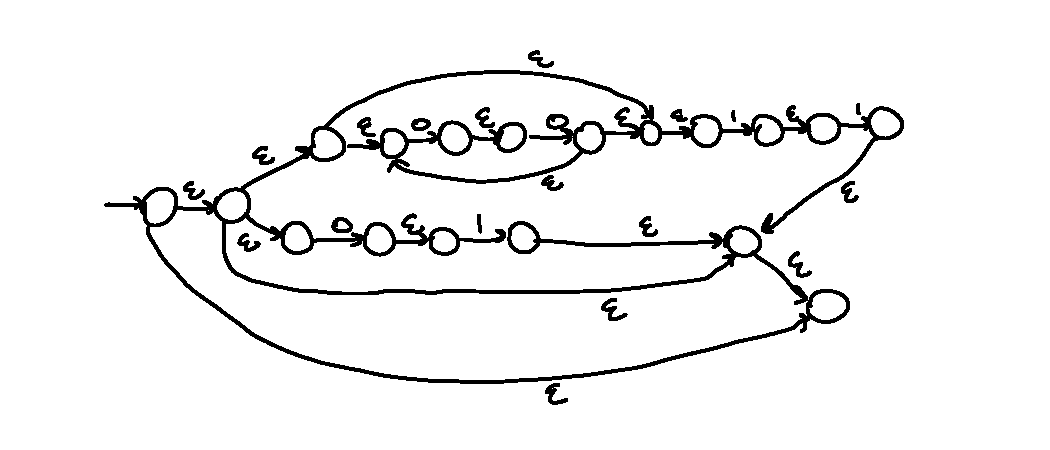
\includegraphics[scale=0.9]{Images/1-19-2b.pdf}
					\caption{AFND, creado con \textit{Xournal}}
					\label{19-2b}
				\end{figure}
		\end{enumerate}
	\end{problem}
\end{mdframed}












\begin{mdframed}[style = warning]
	\begin{problem}
		($1.21$) 	
		\begin{enumerate}[a)]
			\item Dado el AFD, se crean las dos "ecuaciones" que lo representan:
				\begin{align*}
					1 &= a1|b2 \\
					2 &= a2|b1|\lambda
				\end{align*}
				Las cuales, en base a las reglas llevan a la siguiente expresión regular $\boxed{(a^*ba^*b)^*}$
			\item Ahora, para este autómata, se tiene
				\begin{align*}
					1 &= (a|b)2 \\
					2 &= a2|b3 \\
					3 &= a1|b2
				\end{align*}
			Lo que da la sigueinte RE $\boxed{(a|b)((a^*ba)b)^*}$
		\end{enumerate}
	\end{problem}
\end{mdframed}







\section*{Jurado}








\begin{mdframed}[style = warning]
	\begin{problem}
		($3.1$) 	
		\begin{enumerate}[a)]
			\item Para $(a|b)^*c$. Definiendo un subalfabeto $\Sigma ' \subset \Sigma$, la primera parte son todas las palabras generadas por dicho alfabeto. Entonces, el lenguaje generado es:
				$$L = \{ xc: x\in \Sigma '^*, \Sigma ' = \{ a,b \} \}$$
			\item Para $(aa^+)(bb^*)$. Se tiene:
				$$L = \{ aa^nbb^m: n\geq 1, m\geq 0 \}$$
			\item Para $(aa^+)|(bb^*)$. Se tiene:
				$$L = \{ aa^n,bb^m: n\geq 1, m\geq 0 \}$$
			\item Para $a^* b^* c^*$. Es claro que:
				$$L = \{ a^nb^mc^k, n,m,k \geq 0 \}$$
		\end{enumerate}
	\end{problem}
\end{mdframed}

















\begin{mdframed}[style = warning]
	\begin{problem}
		($3.2$) 	
		\begin{enumerate}[a)]
			\item Para generar solo cadenas de longitud par, de $a$'s, se tiene la siguiente expresión regular
				$$(a^2)^*$$
			\item Para longitud impar, es practicamente lo mismo, pero, con una $a$ extra:
				$$a(a^2)^*$$
			\item Para generar siempre cadenas de longitud impar y todas las letras intercaladas, es necesario utilizar la clausura positiva, para asegurar la cadena alternante de menor longitud. Por lo que:
				$$(aba|bab)^+$$
		\end{enumerate}
	\end{problem}
\end{mdframed}











































